\documentclass[12pt,a4paper,oneside]{ctexbook}
\usepackage[left=2cm, right=2cm, top=3cm, bottom=3cm]{geometry}

\usepackage{amsmath}
\usepackage{amssymb}
\usepackage{amsthm}
\usepackage[colorlinks=true, linkcolor=black, citecolor=black]{hyperref}

\theoremstyle{definition}
\theoremstyle{remark}
\newtheorem*{solution}{解析} 

\usepackage{pdfpages}

\usepackage{amsmath}
\usepackage{amssymb}
\usepackage{amsthm}
\usepackage[colorlinks=true, linkcolor=black, citecolor=black]{hyperref}

\setCJKmainfont{fonts/Songti.ttf}
\setCJKsansfont{fonts/Heiti.ttf}
\usepackage{unicode-math}
\setmathfont{NewComputerModernMath} 

\usepackage{pdfpages}

\usepackage{tikz}
\usetikzlibrary{positioning, calc, shapes.geometric} 

\usepackage{tasks}
\usepackage{xparse}
\usepackage[most]{tcolorbox}
\tcbuselibrary{skins, breakable}

\settasks{
	label = \Alph*.,          
	label-width = 1.8em,     
	item-indent = 2.3em,    
	label-offset = 0.5em,   
	column-sep=2em           
}

\newcounter{choicecounter}

\newcommand{\knowledgepointicon}{
	\tikz[baseline=-0.1ex] \node[
	fill=blue!60!cyan,
	shape=diamond,
	aspect=0.7,
	inner sep=1.5pt
	] {};
}

\NewDocumentEnvironment{choice}{m m}{
	\par\addvspace{\medskipamount}
	\stepcounter{choicecounter}
	\begin{tcolorbox}[
		enhanced,
		breakable, 
		frame hidden, 
		borderline west={1.5pt}{0pt}{teal}, 
		colback=white, 
		left=4mm, 
		right=2mm,
		top=2pt,
		bottom=2pt,
		boxsep=0pt, 
		before upper={
			\noindent 
			\textbf{\color{teal}习题 \arabic{choicecounter}} 
			\hfill 
			\knowledgepointicon~\text{#2} \quad 
			{\color{teal!70!blue}[\ \textbf{#1}\ ]} 
			\par\vspace{1ex}
		}
		]
	}{
	\end{tcolorbox}
}

\usepackage{xparse} 

\NewDocumentEnvironment{exercise}{ >{\SplitArgument{1}{}} O{} m m }{
	
}{\relax} % 先定义一个空的,防止报错

\RenewDocumentEnvironment{exercise}{ O{} g g }{% O{}=>[note], g=>{score}, g=>{topic}
	\par\addvspace{\medskipamount}
	\stepcounter{choicecounter}
	\begin{tcolorbox}[
		enhanced, breakable, frame hidden,
		borderline west={1.5pt}{0pt}{teal},
		colback=white,
		left=4mm, right=2mm, top=2pt, bottom=2pt, boxsep=0pt,
		fonttitle=\bfseries,
		% 标题
		title={
			\color{teal}题目 \thechoicecounter % 始终显示题目编号
			% 如果第一个可选参数 (补充说明) 存在, 则显示它
			\IfValueT{#1}{\ (#1)}
			% 如果第二个参数 (分数) 存在, 则显示它
			\IfValueT{#2}{\ (本题 #2 分)}%
			\hfill % 
			% 如果第三个参数 (考点) 存在, 则显示它
			\IfValueT{#3}{\knowledgepointicon~\textcolor{black}{#3}}
		}
		]
	}{
	\end{tcolorbox}
}

\renewenvironment{solution}{
	\par\addvspace{\medskipamount}
	\begin{tcolorbox}[
		enhanced, breakable,
		frame hidden, 
		borderline west={1.5pt}{0pt}{teal}, 
		colback=white, 
		left=4mm, right=2mm, top=2pt, bottom=2pt, boxsep=0pt,
		before upper={ 
			\noindent\textbf{\color{teal}解析}\par\vspace{0.5ex}
		}
		]
	}{
	\end{tcolorbox}
}

\newtcolorbox{note}[1][]{
	enhanced, breakable,
	frame hidden, 
	borderline west={1.5pt}{0pt}{orange}, 
	colback=white, 
	left=4mm, right=2mm, top=2pt, bottom=2pt, boxsep=0pt,
	before upper={ 
		\noindent\textbf{\color{orange}注}\par\vspace{0.5ex}
	},
	#1
}

\begin{document}
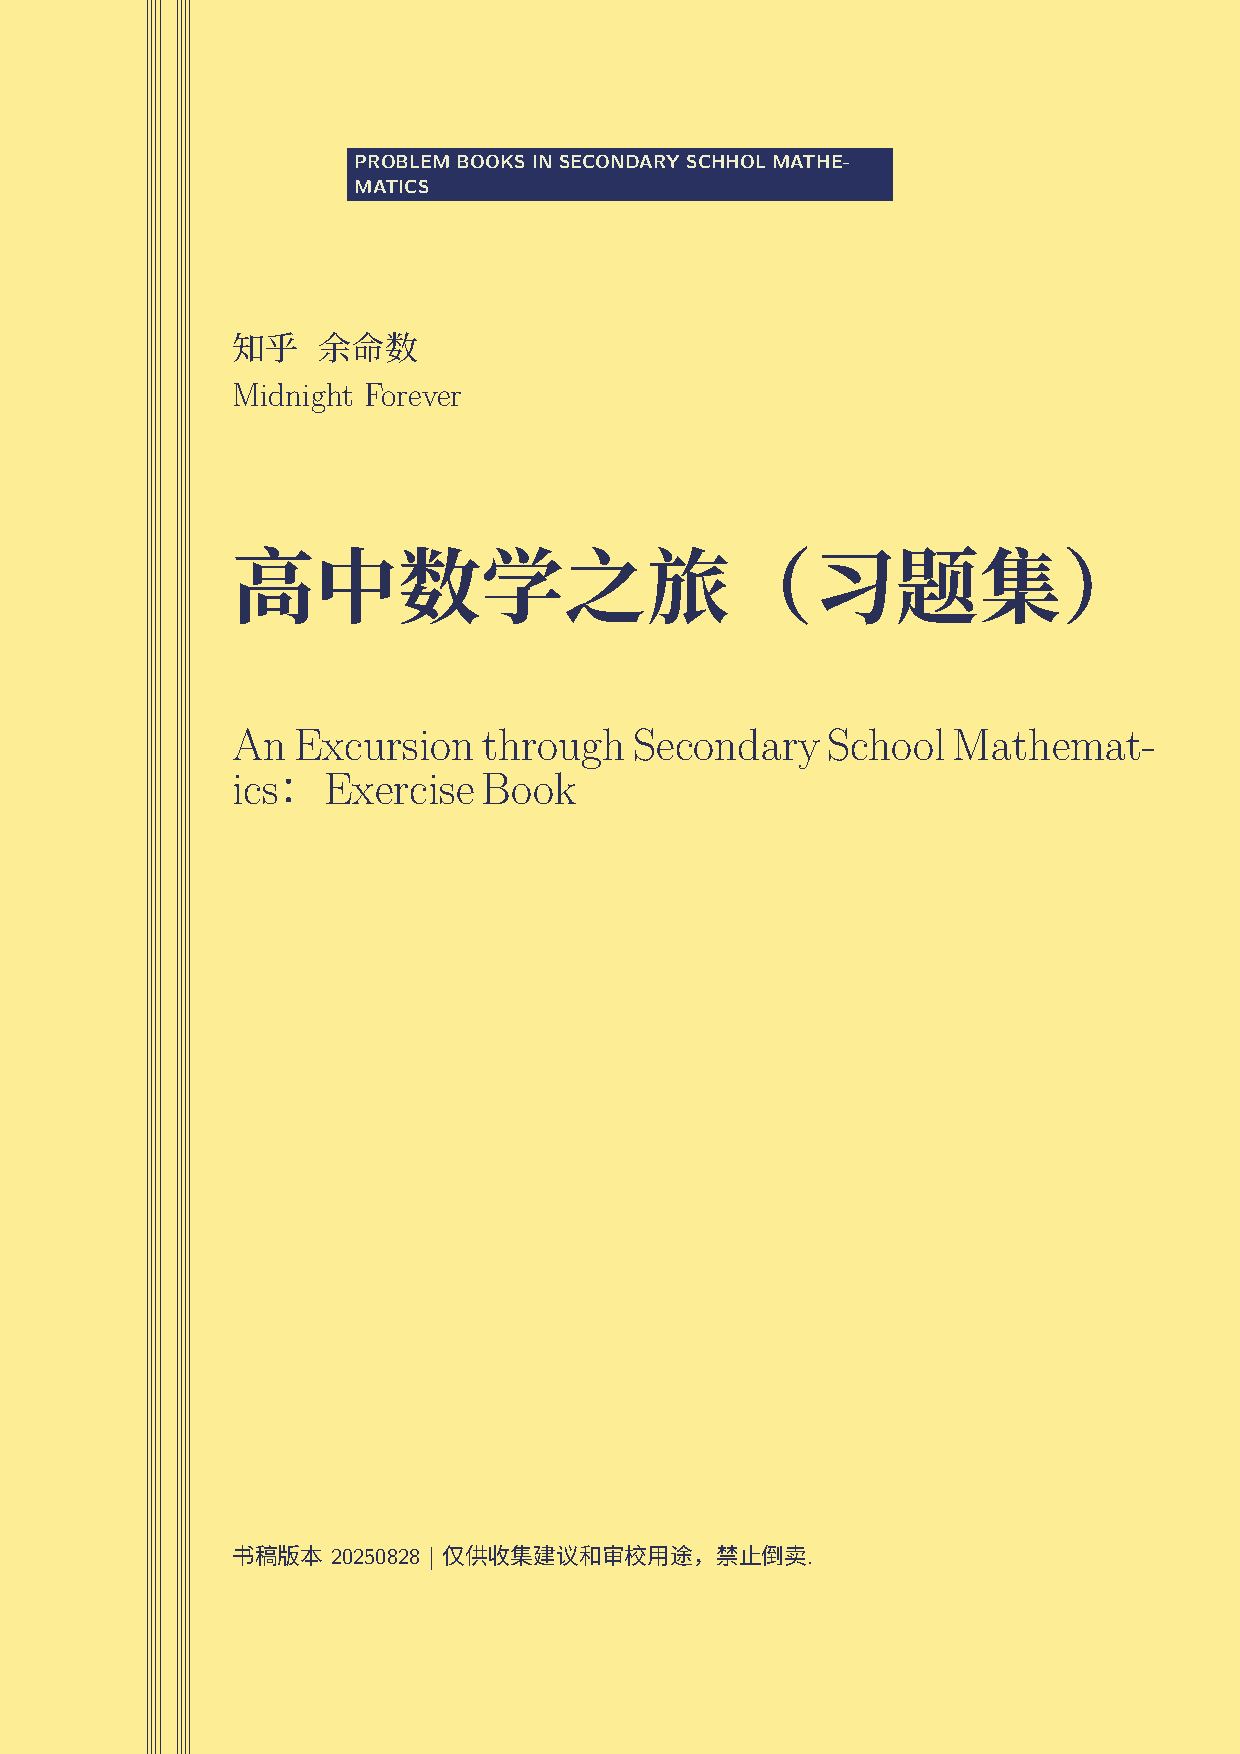
\includepdf[pages=1]{cover.pdf}

{ 
	\thispagestyle{empty} 
	\begin{titlepage}
		\thispagestyle{empty} 
		\begin{flushleft}
			\vspace*{2cm}
			
			{\large
				知乎@余命数 \\
				Midnight Forever
			}
			
			\vspace{4cm}
			
			{\fontsize{36}{44}\selectfont\bfseries 高中数学之旅(习题集)}\\[2cm]

			{\fontsize{22}{28}\selectfont An Excursion through Secondary School Mathematics: Exercise Book}

			\vspace{2cm}

			\vfill

			{\small
				最后更新: \today \\
				书稿版本,禁止修改、倒卖等任何侵犯作者著作权的行为.
			}
		\end{flushleft}
	\end{titlepage}
}

\pagenumbering{roman}
	
	\frontmatter
	\pagestyle{plain}
	\tableofcontents
	
	\mainmatter
	\chapter{集合和逻辑用语}
\setcounter{choicecounter}{0} 

\subsection*{A组}

\begin{choice}{}{量词命题的否定}
	已知命题 $p: \exists x \in \mathbb{N}, x^2 \le 0$,则 $\neg p$ 为
	\begin{tasks}(2)
		\task $\exists x \in \mathbb{N}, x^2 \le 0$
		\task $\exists x \in \mathbb{N}, x^2 > 0$
		\task $\forall x \in \mathbb{N}, x^2 > 0$
		\task $\forall x \in \mathbb{N}, x^2 \ge 0$
	\end{tasks}
\end{choice}

\begin{choice}{}{集合的补集与交集}
	{(2023 秋 • 高一 • 重庆永川区 • 月考校考)} 设集合 $A=\{x|x<2 \text{或} x \ge 4\}, B=\{x|x<a\}$,若 $(\complement_U A) \cap B \neq \emptyset$,则 $a$ 的取值范围是
	\begin{tasks}(2)
		\task $a < 2$
		\task $a > 2$
		\task $a \le 4$
		\task $a \ge 4$
	\end{tasks}
\end{choice}

\begin{choice}{}{集合的交集与子集个数}
	已知集合 $A=\{(x,y) | x,y \in \mathbb{Z}, \text{且 } xy=4\}, B=\{(x,y) | x \le y\}$,则 $A \cap B$ 的子集的个数为
	\begin{tasks}(4)
		\task 3
		\task 4
		\task 8
		\task 16
	\end{tasks}
\end{choice}


\subsection*{B组}

\begin{choice}{}{充分必要条件}
	{(2023 秋 • 高一 • 山东烟台 • 月考校考)} 下列说法错误的是
	\begin{tasks}(1)
		\task “$A \cap B = B$” 是 “$B = \emptyset$” 的必要不充分条件
		\task “$x=3$” 的一个充分不必要条件是 “$x^2-2x-3=0$”
		\task “$|x|=1$” 是 “$x=1$” 的必要不充分条件
		\task “$m$ 是实数” 的一个充分不必要条件是 “$m$ 是有理数”
	\end{tasks}
\end{choice}

\begin{choice}{}{全称命题的否定}
	若命题 “$\forall x \in \mathbb{R}, 1-x^2 \le m$” 是假命题,则实数 $m$ 的取值范围是
	\begin{tasks}(2)
		\task $(-\infty, 1)$
		\task $(-\infty, 1]$
		\task $(1, +\infty)$
		\task $[1, +\infty)$
	\end{tasks}
\end{choice}

\begin{choice}{}{充分不必要条件的应用}
	若 “$x=2$” 是 “$m^2x^2 - (m+3)x + 4 = 0$” 的充分不必要条件,则实数 $m$ 的值为
	\begin{tasks}(2)
		\task 1
		\task $-\frac{1}{2}$
		\task $-\frac{1}{2}$ 或 1
		\task -1 或 $-\frac{1}{2}$
	\end{tasks}
\end{choice}

\begin{choice}{}{集合的补集与互异性}
	设全集 $U=\{1,2,3,4,5\}$,集合 $A=\{1,a,b\}, B=\{4, a-b\}$.若 $\complement_U A = B$,则 $a,b$ 的值分别为
	\begin{tasks}(2)
		\task 3,2
		\task 4,3
		\task 3,2 或 5,3
		\task 5,2 或 5,3
	\end{tasks}
\end{choice}


\subsection*{C组}

\begin{choice}{}{新定义集合与元素互异性}
	{(2024 秋 • 高一 • 福建龙岩 • 开学考试校考)} 定义集合 $A \otimes B = \{x | x=\sqrt{a^2+b^2}, a \in A, b \in B\}$,若 $A=\{n, -1\}, B=\{\sqrt{2}, 1\}$,且集合 $A \otimes B$ 中有 3 个元素,则由实数 $n$ 的所有取值组成的集合的非空真子集的个数为
	\begin{tasks}(4)
		\task 2
		\task 6
		\task 14
		\task 15
	\end{tasks}
\end{choice}

\subsection*{德摩根定律与容斥原理}

\subsubsection*{A组}

\begin{exercise}{5}{集合的并集与补集运算}
	\textbf{(填空题)} 已知全集 $U=\{x \in \mathbb{Z} \mid -3 \le x \le 3\}$, 集合 $A=\{-2, 1, 2\}$, $B=\{-1, 0, 1\}$. 求 $\complement_U(A \cup B) = $ \rule{3cm}{0.5pt}.
\end{exercise}

\begin{exercise}{10}{容斥原理初步应用}
	\textbf{(解答题)} 某班有50名学生,参加数学兴趣小组的有25人,参加物理兴趣小组的有22人,两个小组都参加的有10人.问:
	\begin{enumerate}
		\item 至少参加一个兴趣小组的学生有多少人?
		\item 两个小组都没有参加的学生有多少人?
	\end{enumerate}
\end{exercise}

\subsubsection*{B组}

\begin{exercise}{12}{德摩根定律与一元二次不等式}
	\textbf{(解答题)} 设全集 $U=\mathbb{R}$, 集合 $A=\{x|x \le -1 \text{ 或 } x \ge 4\}$, $B=\{x| x^2-3x-4<0\}$.
	\begin{enumerate}
		\item 求集合 $B$;
		\item 利用德摩根定律,求 $\complement_U(A \cap B)$.
	\end{enumerate}
\end{exercise}

\begin{exercise}{12}{容斥原理的逆向应用}
	\textbf{(解答题)} 某次考试中,50名学生参加了数学和物理两科.已知数学成绩及格的有40人,物理成绩及格的有31人,两科都不及格的有4人.问这次考试中:
	\begin{enumerate}
		\item 两科都及格的学生有多少人?
		\item 恰好只有一科及格的学生有多少人?
	\end{enumerate}
\end{exercise}


\subsubsection*{C组}

\begin{exercise}{12}{三集合容斥原理}
	\textbf{(解答题)} 某新闻机构就A, B, C三个热点话题对100人进行调查,结果显示:关注A的有45人,B的有55人,C的有60人;同时关注A和B的有25人,A和C的有20人,B和C的有30人;三个话题都关注的有10人.问:
	\begin{enumerate}
		\item 至少关注一个话题的人数是多少?
		\item 恰好只关注一个话题的人数是多少?
	\end{enumerate}
\end{exercise}
	\chapter{解三角形}
\setcounter{choicecounter}{0} 

\section{取值范围}
\subsection{知识回顾}
解决问题的第一步,是将题目中多变量换成单变量. 这是化繁为简、确立解题方向的关键.
\begin{itemize}
	\item \textbf{若表达式含边或边的比例},优先考虑使用\textbf{正弦定理} ($a=2R\sin A, b=2R\sin B, \dots$),将边长转化为对应角的正弦,实现“\textbf{边化角}”.
	\item \textbf{若表达式含边的平方},或已知条件为“两边一夹角” (SAS) / “三边” (SSS),则\textbf{余弦定理}是构造关系式的不二之选. 
	\item \textbf{利用内角和定理} $A+B+C=\pi$ 消去多余的角变量,是实现“变量化归”的最后一步.
\end{itemize}

牢记定义域,这是最关键也最容易被忽略的一步. 三角形中的角并非任意取值,其范围受到严格的内在约束. 忘记定义域,犹如脱缰之马,所得结论往往谬以千里.
\begin{itemize}
	\item \textbf{基本约束}:三角形的任意内角都必须在 $(0, \pi)$ 范围内.
	\item \textbf{结构约束}:例如,若已将其他角用变量角 $B$ 表示为 $A=\frac{\pi}{2}-2B, C=\frac{\pi}{2}+B$,则必须同时满足 $B>0, A>0, C>0$,即
	$\begin{cases} B>0 \\ \frac{\pi}{2}-2B>0 \\ \frac{\pi}{2}+B>0 \end{cases}$
	解出这些不等式组,才能得到 $B$ 的最终有效范围.
	\item \textbf{附加约束}:题目若明确指出是“锐角三角形”、“钝角三角形”等,则需要增加所有角小于 $\frac{\pi}{2}$ 或某个角大于 $\frac{\pi}{2}$ 的限制条件.
\end{itemize}

完成前两步后,问题就从一个复杂的几何问题,转化为了我们极为熟悉的、求函数在特定区间上最值的常规问题. 此时,我们有多种工具可供选择.
\begin{itemize}
	\item \textbf{辅助角公式}:对于形如 $y=a\sin x + b\cos x$ 的函数,此法是首选.
	\item \textbf{二次函数配方法}:对于形如 $y=a\sin^2 x + b\sin x + c$ 的函数,可通过换元法转化为二次函数在闭区间上的最值问题.
	\item \textbf{求导}:对于更复杂的三角函数,求导是判断其单调性、寻找极值点的最通用、最强大的方法.
\end{itemize}

\subsection{习题集}
\subsubsection{取值范围}
\begin{exercise}[2022 年全国新高考 I 卷第 18 题]
	记 $\triangle ABC$ 的内角 $A,B,C$ 的对边分别为 $a,b,c$, 已知 $\frac{\cos A}{1+\sin A} = \frac{\sin 2B}{1+\cos 2B}$.
	\begin{enumerate}
		\item[(1)] 若 $C = \frac{2\pi}{3}$, 求 $B$;
		\item[(2)] 求 $\frac{a^2+b^2}{c^2}$ 的最小值.
	\end{enumerate}
\end{exercise}

\begin{exercise}[2023 年衡水中学第三次综合素养评价第 18 题]
	已知在 $\triangle ABC$ 的内角 $A,B,C$ 所对边分别为 $a,b,c$, 且 $a=b+2b\cos C$.
	\begin{enumerate}
		\item[(1)] 求证: $C=2B$;
		\item[(2)] 求 $\frac{a+c}{b}$ 的取值范围.
	\end{enumerate}
\end{exercise}

\begin{exercise}
	已知 $\triangle ABC$ 的面积为 $S$, 角 $A,B,C$ 所对的边分别为 $a,b,c$.点 $O$ 为 $\triangle ABC$ 的内心, $b = 2\sqrt{3}$ 且 $S = \frac{\sqrt{3}}{4}(a^2+c^2-b^2)$.
	\begin{enumerate}
		\item[(1)] 求 $B$ 的大小;
		\item[(2)] 求 $\triangle AOC$ 的周长的取值范围.
	\end{enumerate}
\end{exercise}

\begin{exercise}
	在锐角 $\triangle ABC$ 中, 角 $A, B, C$ 所对应的边分别为 $a, b, c$, 已知 $\frac{\sin A - \sin B}{\sqrt{3}a - c} = \frac{\sin C}{a+b}$.
	\begin{enumerate}
		\item[(1)] 求角 $B$ 的值;
		\item[(2)] 若 $a=2$, 求 $\triangle ABC$ 的周长的取值范围.
	\end{enumerate}
\end{exercise}

\subsubsection{面积问题}
\begin{exercise}[2023 浙江省十校联盟第三次联考第 18 题]
	在 $\triangle ABC$ 中, $D$ 为边 $BC$ 上一点, $DC = 3, AD = 5, AC = 7, \angle DAC = \angle ABC$.
	\begin{enumerate}
		\item[(1)] 求 $\angle ADC$ 的大小;
		\item[(2)] 求 $\triangle ABC$ 的面积.
	\end{enumerate}
\end{exercise}
	
	\chapter{参考答案}
	\section{集合和逻辑用语}

\subsection*{A组}

\subsubsection*{题目 1}
\begin{solution}
	\textbf{答案 C}
	
	本题考查全称量词命题与存在量词命题的否定关系.否定一个量词命题,遵循“改量词,否结论”的原则.
	原命题 $p$ 为一个存在量词命题,其逻辑形式为 $\exists x \in M, P(x)$.
	
	其否定的一般形式为:
	\[ \neg (\exists x \in M, P(x)) \iff \forall x \in M, \neg P(x) \]
	在本题中,量词 $\exists$ (存在) 的否定是 $\forall$ (任意).
	原结论 $P(x)$ 为 $x^2 \le 0$,其否定 $\neg P(x)$ 为 $x^2 > 0$.
	
	故 $\neg p$ 为 $\forall x \in \mathbb{N}, x^2 > 0$.
\end{solution}

\begin{note}
	选项 D 中,$x^2 \ge 0$ 在自然数范围内是恒成立的,但它并非 $x^2 \le 0$ 的严格否定.一个结论的否定是其逻辑补集,而非简单的反义关系.对于实数 $y$,$y \le 0$ 的否定是 $y>0$.
\end{note}

\subsubsection*{题目 2}
\begin{solution}
	\textbf{答案 B}
	
	本题的核心思想是将抽象的集合运算转化为直观的数轴位置关系.
	首先,根据集合 $A$ 的定义,确定其在全集 $U=\mathbb{R}$ 下的补集.
	\[ A = \{x|x<2 \text{ 或 } x \ge 4\} = (-\infty, 2) \cup [4, +\infty) \]
	其补集为数轴上未被覆盖的部分:
	\[ \complement_U A = \{x|2 \le x < 4\} = [2, 4) \]
	集合 $B$ 的定义为:
	\[ B = \{x|x<a\} = (-\infty, a) \]
	题目条件为 $(\complement_U A) \cap B \neq \emptyset$,即区间 $[2, 4)$ 与 $(-\infty, a)$ 的交集不为空.
	为满足此条件,区间 $(-\infty, a)$ 的右端点 $a$ 必须大于区间 $[2,4)$ 的左端点 $2$.
	因此,可得 $a > 2$.
\end{solution}

\subsubsection*{题目 3}
\begin{solution}
	\textbf{答案 D}
	
	解题分为两个步骤:首先确定交集 $A \cap B$ 的所有元素,然后利用子集个数公式求解.
	
	第一步,列举集合 $A$ 的所有元素.$A$ 的元素是满足 $xy=4$ 的整数坐标点 $(x,y)$.
	\[ A = \{(1,4), (4,1), (-1,-4), (-4,-1), (2,2), (-2,-2)\} \]
	第二步,从 $A$ 中筛选出满足集合 $B$ 条件 ($x \le y$) 的元素.
	\[ A \cap B = \{(1,4), (-4,-1), (2,2), (-2,-2)\} \]
	集合 $A \cap B$ 中含有 4 个元素.
	
	一个含有 $n$ 个元素的有限集合,其子集的个数为 $2^n$.
	本题中 $n=4$,故子集个数为 $2^4 = 16$.
\end{solution}

\subsection*{B组}

\subsubsection*{题目 4}
\begin{solution}
	\textbf{答案 D}
	
	本题考查充分条件与必要条件的判断.核心方法是将命题间的逻辑关系转化为集合间的包含关系:若 $p \Rightarrow q$,则 $p$ 对应的集合是 $q$ 对应集合的子集.
	
	A. “$A \cap B = B$” 等价于 $B \subseteq A$.“$B=\emptyset$” 能够推出 $B \subseteq A$,但反之不成立.因此,“$B \subseteq A$” 是 “$B=\emptyset$” 的必要不充分条件.该说法正确.
	
	B. “$x=3$” 对应集合 $\{3\}$.“$x^2-2x-3=0$” 对应解集 $\{3, -1\}$.因为 $\{3\} \subsetneq \{3, -1\}$,所以前者是后者的充分不必要条件.该说法正确.
	
	C. “$|x|=1$” 对应集合 $\{1, -1\}$.“$x=1$” 对应集合 $\{1\}$.因为 $\{1\} \subsetneq \{1, -1\}$,所以前者是后者的必要不充分条件.该说法正确.
	
	D. 命题 $p$: “$m$ 是有理数”,对应集合 $\mathbb{Q}$.命题 $q$: “$m$ 是实数”,对应集合 $\mathbb{R}$.因为 $\mathbb{Q} \subsetneq \mathbb{R}$,所以 $p$ 是 $q$ 的充分不必要条件.原说法颠倒了主次,故错误.
\end{solution}

\subsubsection*{题目 5}
\begin{solution}
	\textbf{答案 A}
	
	一个全称量词命题为假,其逻辑等价于它的否定形式(一个存在量词命题)为真.
	设原命题为 $P: \forall x \in \mathbb{R}, 1-x^2 \le m$.
	
	由于命题 $P$ 为假,其否定命题 $\neg P$ 必为真.
	\[ \neg P: \exists x \in \mathbb{R}, \neg(1-x^2 \le m) \implies \exists x \in \mathbb{R}, 1-x^2 > m \]
	该存在量词命题为真,意味着 $m$ 必须小于函数 $f(x) = 1-x^2$ 的最大值.
	函数 $f(x)=1-x^2$ 是一个开口向下的二次函数,其顶点为最大值点.
	\[ f(x)_{\max} = f(0) = 1 \]
	因此,实数 $m$ 的取值范围必须是 $m < 1$,即 $m \in (-\infty, 1)$.
\end{solution}

\subsubsection*{题目 6}
\begin{solution}
	\textbf{答案 B}
	
	命题“$p$ 是 $q$ 的充分不必要条件”包含两层含义,必须同时满足:
	\begin{itemize}
		\item \textbf{充分性}: $p \Rightarrow q$.
		\item \textbf{不必要性}: $q \not\Rightarrow p$.
	\end{itemize}
	设 $p: x=2$,$q: m^2x^2 - (m+3)x + 4 = 0$.
	
	\textbf{检验充分性}:
	将 $x=2$ 代入方程 $q$ 中,方程必须成立.
	\[ 4m^2 - 2(m+3) + 4 = 0 \implies 2m^2 - m - 1 = 0 \]
	因式分解得 $(2m+1)(m-1) = 0$,解得 $m=1$ 或 $m=-\frac{1}{2}$.
	
	\textbf{检验不必要性}:
	方程 $q$ 的解集 $S$ 必须真包含 $\{2\}$,即 $S \neq \{2\}$.
	\begin{itemize}
		\item 当 $m=1$ 时,方程为 $x^2 - 4x + 4 = 0$,解集 $S=\{2\}$.此时 $q \Rightarrow p$ 成立,不满足“不必要”条件,故舍去.
		\item 当 $m=-\frac{1}{2}$ 时,方程为 $\frac{1}{4}x^2 - \frac{5}{2}x + 4 = 0$,即 $x^2 - 10x + 16 = 0$.解集 $S=\{2, 8\}$.此时 $S \neq \{2\}$,满足“不必要”条件.
	\end{itemize}
	综上,唯一满足条件的实数 $m$ 的值为 $-\frac{1}{2}$.
\end{solution}

\subsubsection*{题目 7}
\begin{solution}
	\textbf{答案 D}
	
	条件 $\complement_U A = B$ 是解题的关键,它等价于以下两个条件同时成立:
	\[ A \cup B = U \quad \text{且} \quad A \cap B = \emptyset \]
	根据题意:
	$U=\{1,2,3,4,5\}$
	$A=\{1,a,b\}$
	$B=\{4, a-b\}$
	
	由 $A \cup B = U$,可得:
	\[ \{1,a,b\} \cup \{4, a-b\} = \{1, a, b, 4, a-b\} = \{1,2,3,4,5\} \]
	比较两集合,可知无序集合 $\{a, b, a-b\}$ 必须与 $\{2,3,5\}$ 相等.
	同时,集合 A 和 B 的元素必须满足互异性.
	
	我们通过分类讨论来寻找 $a,b$ 的取值:
	\begin{itemize}
		\item \textbf{情况一:} 设 $a=5, b=2$.则 $a-b = 3$.此时 $\{a,b,a-b\} = \{5,2,3\}$ 与 $\{2,3,5\}$ 匹配.
		检验:$A=\{1,5,2\}, B=\{4,3\}$.此时 $\complement_U A = \{3,4\}=B$,符合题意.
		\item \textbf{情况二:} 设 $a=5, b=3$.则 $a-b = 2$.此时 $\{a,b,a-b\} = \{5,3,2\}$ 与 $\{2,3,5\}$ 匹配.
		检验:$A=\{1,5,3\}, B=\{4,2\}$.此时 $\complement_U A = \{2,4\}=B$,符合题意.
	\end{itemize}
	其他组合(如 $a=3,b=2$ 时 $a-b=1$,与$A$中元素重复)均不满足条件.
	因此,$a,b$ 的值为 5,2 或 5,3.
\end{solution}

\subsection*{C组}

\subsubsection*{题目 8}
\begin{solution}
	\textbf{答案 B}
	
	本题综合考查了新定义集合的理解、集合元素的互异性以及子集个数的计算.
	
	\textbf{1. 构造集合 $A \otimes B$}
	根据定义,$A=\{n, -1\}, B=\{\sqrt{2}, 1\}$.
	\[ A \otimes B = \{\sqrt{n^2 + (\sqrt{2})^2}, \sqrt{n^2 + 1^2}, \sqrt{(-1)^2 + (\sqrt{2})^2}, \sqrt{(-1)^2 + 1^2}\} \]
	化简得:
	\[ A \otimes B = \{\sqrt{n^2+2}, \sqrt{n^2+1}, \sqrt{3}, \sqrt{2}\} \]
	
	\textbf{2. 应用元素个数条件}
	已知 $|A \otimes B| = 3$.由于上式给出了 4 个表达式,根据集合元素的互异性,其中必有两个表达式的值相等.
	注意到 $\sqrt{n^2+2} > \sqrt{n^2+1}$ 且 $\sqrt{3} > \sqrt{2}$,因此相等的只可能是一个含 $n$ 的项与一个常数项.
	
	分类讨论:
	\begin{itemize}
		\item 若 $\sqrt{n^2+1} = \sqrt{2} \implies n^2=1 \implies n=\pm 1$.此时 $\sqrt{n^2+2}=\sqrt{3}$,集合为 $\{\sqrt{2}, \sqrt{3}\}$,仅有 2 个元素,不合题意.
		\item 若 $\sqrt{n^2+1} = \sqrt{3} \implies n^2=2 \implies n=\pm \sqrt{2}$.此时 $\sqrt{n^2+2}=\sqrt{4}=2$,集合为 $\{2, \sqrt{3}, \sqrt{2}\}$,有 3 个元素,符合题意.
		\item 若 $\sqrt{n^2+2} = \sqrt{2} \implies n^2=0 \implies n=0$.此时 $\sqrt{n^2+1}=1$,集合为 $\{1, \sqrt{3}, \sqrt{2}\}$,有 3 个元素,符合题意.
		\item 若 $\sqrt{n^2+2} = \sqrt{3} \implies n^2=1$, 情况同第一类,不符.
	\end{itemize}
	
	\textbf{3. 计算子集个数}
	由上可知,实数 $n$ 的所有取值组成的集合为 $S_n = \{-\sqrt{2}, 0, \sqrt{2}\}$.
	该集合有 $k=3$ 个元素.
	非空真子集的个数为 $2^k - 2 = 2^3 - 2 = 6$.
\end{solution}

\subsection*{专题训练参考答案与解析}

\subsubsection*{题目 9}
\begin{solution}
	\textbf{答案} $\{-3, 3\}$
	
	本题考查有限集合的补集运算.
	
	\textbf{方法一:直接法}
	首先确定全集 $U$ 和并集 $A \cup B$.
	\[ U = \{-3, -2, -1, 0, 1, 2, 3\} \]
	\[ A \cup B = \{-2, 1, 2\} \cup \{-1, 0, 1\} = \{-2, -1, 0, 1, 2\} \]
	$\complement_U(A \cup B)$ 即为在 $U$ 中但不在 $A \cup B$ 中的元素所构成的集合.
	\[ \complement_U(A \cup B) = \{-3, 3\} \]
	
	\textbf{方法二:德摩根定律}
	根据德摩根定律,$\complement_U(A \cup B) = (\complement_U A) \cap (\complement_U B)$.
	\[ \complement_U A = \{-3, -1, 0, 3\} \]
	\[ \complement_U B = \{-3, -2, 2, 3\} \]
	两补集的交集为:
	\[ (\complement_U A) \cap (\complement_U B) = \{-3, 3\} \]
\end{solution}

\subsubsection*{题目 10}
\begin{solution}
	本题是容斥原理的直接应用.设参加数学兴趣小组的学生集合为 $M$,参加物理兴趣小组的学生集合为 $P$.
	根据题意,已知信息为:
	\[ |M| = 25, \quad |P| = 22, \quad |M \cap P| = 10 \]
	(1) \textbf{至少参加一个兴趣小组的人数},即求 $|M \cup P|$.
	根据容斥原理公式:
	\[ |M \cup P| = |M| + |P| - |M \cap P| = 25 + 22 - 10 = 37 \text{ (人)} \]
	
	(2) \textbf{两个小组都没有参加的人数}.
	设全班学生为全集 $U$,则所求人数为 $|\complement_U(M \cup P)|$.
	\[ |\complement_U(M \cup P)| = |U| - |M \cup P| = 50 - 37 = 13 \text{ (人)} \]
\end{solution}

\subsubsection*{题目 11}
\begin{solution}
	本题将德摩根定律与一元二次不等式的求解相结合.
	
	(1) \textbf{求集合 B}
	解不等式 $x^2-3x-4<0$.
	因式分解得 $(x-4)(x+1)<0$,解得 $-1 < x < 4$.
	\[ B=\{x \mid -1 < x < 4\} = (-1, 4) \]
	
	(2) \textbf{求 $\complement_U(A \cap B)$}
	直接计算 $A \cap B$ 再求补集较为繁琐,应用德摩根定律可以简化运算.
	\[ \complement_U(A \cap B) = (\complement_U A) \cup (\complement_U B) \]
	分别计算两个补集:
	\[ \complement_U A = \{x \mid \neg(x \le -1 \text{ 或 } x \ge 4)\} = \{x \mid -1 < x < 4\} = (-1, 4) \]
	\[ \complement_U B = \{x \mid \neg(-1 < x < 4)\} = \{x \mid x \le -1 \text{ 或 } x \ge 4\} = (-\infty, -1] \cup [4, \infty) \]
	求它们的并集:
	\[ (\complement_U A) \cup (\complement_U B) = (-1, 4) \cup \left( (-\infty, -1] \cup [4, \infty) \right) = \mathbb{R} \]
	因此,$\complement_U(A \cap B) = \mathbb{R}$.
\end{solution}

\subsubsection*{题目 12}
\begin{solution}
	本题是容斥原理的逆向和综合应用.设数学及格的集合为 $M$,物理及格的集合为 $P$.
	已知信息:
	\[ |U|=50, \quad |M|=40, \quad |P|=31 \]
	“两科都不及格”的人数为 4,即 $|\complement_U(M \cup P)|=4$.
	
	(1) \textbf{求两科都及格的人数},即求 $|M \cap P|$.
	首先,由补集信息计算至少有一科及格的人数 $|M \cup P|$.
	\[ |M \cup P| = |U| - |\complement_U(M \cup P)| = 50 - 4 = 46 \]
	再根据容斥原理 $|M \cup P| = |M| + |P| - |M \cap P|$,可得:
	\[ 46 = 40 + 31 - |M \cap P| \]
	\[ |M \cap P| = 71 - 46 = 25 \text{ (人)} \]
	
	(2) \textbf{求恰好只有一科及格的人数}.
	这部分学生等于“至少一科及格”的人数减去“两科都及格”的人数.
	\[ |(M \cup P) \setminus (M \cap P)| = |M \cup P| - |M \cap P| = 46 - 25 = 21 \text{ (人)} \]
\end{solution}

\subsubsection*{题目 13}
\begin{solution}
	本题是三集合容斥原理的经典应用.设关注 A, B, C 话题的人构成的集合分别为 $A, B, C$.
	已知信息:
	\[ |A|=45, |B|=55, |C|=60 \]
	\[ |A \cap B|=25, |A \cap C|=20, |B \cap C|=30 \]
	\[ |A \cap B \cap C|=10 \]
	
	(1) \textbf{求至少关注一个话题的人数},即求 $|A \cup B \cup C|$.
	应用三集合容斥原理公式:
	\begin{align*}
		|A \cup B \cup C| &= (|A|+|B|+|C|) - (|A \cap B|+|A \cap C|+|B \cap C|) + |A \cap B \cap C| \\
		&= (45+55+60) - (25+20+30) + 10 \\
		&= 160 - 75 + 10 \\
		&= 95 \text{ (人)}
	\end{align*}
	
	(2) \textbf{求恰好只关注一个话题的人数}.
	这部分人数等于只关注 A,只关注 B,只关注 C 的人数之和.
	
	只关注A的人数:
	\[ |A \setminus (B \cup C)| = |A| - |A \cap B| - |A \cap C| + |A \cap B \cap C| = 45 - 25 - 20 + 10 = 10 \text{ (人)} \]
	只关注B的人数:
	\[ |B \setminus (A \cup C)| = |B| - |A \cap B| - |B \cap C| + |A \cap B \cap C| = 55 - 25 - 30 + 10 = 10 \text{ (人)} \]
	只关注C的人数:
	\[ |C \setminus (A \cup B)| = |C| - |A \cap C| - |B \cap C| + |A \cap B \cap C| = 60 - 20 - 30 + 10 = 20 \text{ (人)} \]
	
	总人数为 $10 + 10 + 20 = 40$ (人).
\end{solution}
	\section{解三角形}
\subsection{取值范围}

\subsubsection{习题1}
\begin{solution}
	本题的核心数学对象是 $\triangle ABC$,回顾我们所学的知识,一个三角形的\textbf{形状}由其三个内角 $A, B, C$ 决定.由于内角和为 $\pi$,即 $A+B+C=\pi$,,是为其一之约束,因此,一个三角形的形状本质上只有 \textbf{2 个自由度}.我们可以选择任意两个角(例如 $A$ 和 $B$)作为独立的参数,第三个角 $C$ 便随之确定.
	
	题目给出的条件 $\frac{\cos A}{1+\sin A} = \frac{\sin 2B}{1+\cos 2B}$ 是一个满足式条件,而我们的首要任务,就是将这个不咋好看的等式,翻译成一个关于角 $A, B$ 的更简洁的关系式.
	
	因此,我们化简下原式,在等式左边,利用半角公:
	\[
	\frac{\cos A}{1+\sin A} = \frac{\sin(\frac{\pi}{2}-A)}{1+\cos(\frac{\pi}{2}-A)} = \frac{2\sin(\frac{\pi}{4}-\frac{A}{2})\cos(\frac{\pi}{4}-\frac{A}{2})}{2\cos^2(\frac{\pi}{4}-\frac{A}{2})} = \tan\left(\frac{\pi}{4}-\frac{A}{2}\right)
	\]
	等式右边,利用二倍角公式:
	\[
	\frac{\sin 2B}{1+\cos 2B} = \frac{2\sin B \cos B}{1+(2\cos^2 B-1)} = \frac{2\sin B \cos B}{2\cos^2 B} = \tan B
	\]
	因此:
	\[
	\tan\left(\frac{\pi}{4}-\frac{A}{2}\right) = \tan B
	\]
	由于 $A, B \in (0, \pi)$, 可知 $\frac{\pi}{4}-\frac{A}{2} \in (-\frac{\pi}{4}, \frac{\pi}{4})$.在各自的定义域内,正切函数是单调的,故:
	\[
	\frac{\pi}{4}-\frac{A}{2} = B \quad \implies \quad A+2B = \frac{\pi}{2}
	\]
	这个简洁的关系,就是原复杂三角等式背后隐藏的约束.它将三角形形状的 2 个自由度削减为了 \textbf{1 个自由度}.接着,我们只需要确定一个角,整个三角形的形状就完全确定了.
	
	\textbf{对于第 (1) 问:}
	题目给出了构造式条件 $C = \frac{2\pi}{3}$,这提供了消除最后一个自由度的信息.我们现在有两个关于 $A, B, C$ 的线性约束:
	\begin{align*}
		A+B+C &= \pi \quad  \\
		A+2B \qquad &= \frac{\pi}{2} \quad 
	\end{align*}
	将 $C=\frac{2\pi}{3}$ 代入第一个式子,得到 $A+B = \frac{\pi}{3}$.联立方程组:
	\[
	\begin{cases}
		A+2B = \frac{\pi}{2} \\
		A+B = \frac{\pi}{3}
	\end{cases}
	\]
	解得 $B = \frac{\pi}{6}$.至此,三角形的所有角都被唯一确定,问题解决.
	
	\textbf{对于第 (2) 问:}
	此问没有给出额外条件,因此我们需要在由 $A+2B=\frac{\pi}{2}$ 所确定的\textbf{所有可能}的三角形形状中,寻找目标表达式的最小值.这正是用自由度参数表达并求解思想的用武之地.
	
	我们选择角 $B$ 作为描述三角形形状的唯一自由参数.其他角可以用 $B$ 表示:
	\begin{align*}
		A &= \frac{\pi}{2}-2B \\
		C &= \pi - (A+B) = \pi - \left(\left(\frac{\pi}{2}-2B\right)+B\right) = \frac{\pi}{2}+B
	\end{align*}
	为了使 $\triangle ABC$ 成立,所有内角必须为正:
	\[
	A > 0 \implies \frac{\pi}{2}-2B > 0 \implies B < \frac{\pi}{4}
	\]
	\[
	B > 0 \quad \text{且} \quad C = \frac{\pi}{2}+B > 0 \quad (\text{当 } B>0 \text{ 时恒成立})
	\]
	综上,自由参数 $B$ 的取值范围是 $(0, \frac{\pi}{4})$.
	
	目标函数是 $\frac{a^2+b^2}{c^2}$.利用正弦定理,将其从边长语言翻译为角度语言:
	\[
	\frac{a^2+b^2}{c^2} = \frac{\sin^2 A + \sin^2 B}{\sin^2 C}
	\]
	将所有角用参数 $B$ 代入:
	\[
	f(B) = \frac{\sin^2(\frac{\pi}{2}-2B) + \sin^2 B}{\sin^2(\frac{\pi}{2}+B)} = \frac{\cos^2(2B) + \sin^2 B}{\cos^2 B}
	\]
	问题转化为:求函数 $f(B)$ 在区间 $B \in (0, \frac{\pi}{4})$ 上的最小值.
	
	为了简化计算,我们进行变量代换.这是一个典型的换元法应用,其本质是将问题从三角函数空间映射到更易于处理的代数空间.
	令 $x = \sin^2 B$.
	由于 $B \in (0, \frac{\pi}{4})$, 新变量 $x$ 的取值范围是 $(0, \sin^2(\frac{\pi}{4})) = (0, \frac{1}{2})$.
	我们将 $f(B)$ 的表达式完全用 $x$ 来表示:
	\[
	\cos^2 B = 1-\sin^2 B = 1-x \quad \text{且} \quad \cos(2B) = 1-2\sin^2 B = 1-2x
	\]
	代入得到关于 $x$ 的函数 $g(x)$:
	\[
	g(x) = \frac{(1-2x)^2+x}{1-x} = \frac{4x^2-3x+1}{1-x}
	\]
	为求 $g(x)$ 在区间 $(0, \frac{1}{2})$ 上的最小值,我们对其求导:
	\[
	g'(x) = \frac{(8x-3)(1-x) - (4x^2-3x+1)(-1)}{(1-x)^2} = \frac{-4x^2+8x-2}{(1-x)^2}
	\]
	令 $g'(x)=0$, 即 $2x^2-4x+1 = 0$.解得 $x = 1 \pm \frac{\sqrt{2}}{2}$.
	考虑到定义域 $x \in (0, \frac{1}{2})$,我们取驻点 $x_0 = 1 - \frac{\sqrt{2}}{2}$.
	分析可知,当 $x \in (0, x_0)$ 时,$g'(x)<0$;当 $x \in (x_0, \frac{1}{2})$ 时,$g'(x)>0$.因此 $g(x)$ 在 $x=x_0$ 处取得最小值.
	将 $x_0 = 1 - \frac{\sqrt{2}}{2}$ 代入 $g(x)$.为简化计算,先对 $g(x)$ 进行代数变形:
	\[
	g(x) = \frac{-4x(1-x)+(x-1)+2}{1-x} = -4x-1+\frac{2}{1-x}
	\]
	最小值为:
	\begin{align*}
		g\left(1 - \frac{\sqrt{2}}{2}\right) &= -4\left(1-\frac{\sqrt{2}}{2}\right) - 1 + \frac{2}{1-\left(1-\frac{\sqrt{2}}{2}\right)} \\
		&= -4 + 2\sqrt{2} - 1 + \frac{2}{\frac{\sqrt{2}}{2}} \\
		&= -5 + 2\sqrt{2} + 2\sqrt{2} \\
		&= 4\sqrt{2}-5
	\end{align*}\hfill\qedsymbol
\end{solution}

\subsubsection{习题2}
\begin{solution}
	题目给出的核心约束是关于边和角的满足式条件”$a=b+2b\cos C$.为了得到我们想要的关系,我们先利用正弦定理翻译起手,目的是将边长关系翻译为角度关系.
	
	由正弦定理,设 $a=k\sin A, b=k\sin B, c=k\sin C$.代入原式得:
	\[
	k\sin A = k\sin B + 2k\sin B \cos C
	\]
	由于 $k \neq 0$, 两边同除以 $k$ 得:
	\[
	\sin A = \sin B + 2\sin B \cos C
	\]
	在 $\triangle ABC$ 中, $A = \pi-(B+C)$, 故 $\sin A = \sin(\pi-(B+C)) = \sin(B+C)$.代入上式:
	\[
	\sin(B+C) = \sin B + 2\sin B \cos C
	\]
	展开左侧:
	\[
	\sin B \cos C + \cos B \sin C = \sin B + 2\sin B \cos C
	\]
	移项整理得:
	\[
	\cos B \sin C - \sin B \cos C = \sin B
	\]
	左侧恰为差角公式,即 $\sin(C-B) = \sin B$.
	
	由于 $B,C$ 均为三角形内角,故 $B \in (0,\pi), C \in (0,\pi)$.同时 $B+C \in (0,\pi)$, 可得 $C-B \in (-\pi, \pi)$.
	由 $\sin(C-B)=\sin B$ 可得两种可能:
	\begin{itemize}
		\item $C-B = B$, 即 $C=2B$.
		\item $C-B = \pi - B$, 即 $C=\pi$.矛盾.
	\end{itemize}
	因此, $C=2B$.至此,第 (1) 问得证.
	
	第 (1) 问的结论 $C=2B$ 极大地简化了问题,它将三角形形状的自由度从 2 降至 1.我们可以选择角 $B$ 作为唯一的自由参数来描述所有满足条件的三角形.
	
	首先,我们将所有角用参数 $B$ 表示,也即所谓的选定变量,或者说是归一思想:
	\[
	C=2B, \quad A = \pi - (B+C) = \pi - 3B
	\]
	为保证 $A,B,C$ 构成一个三角形,所有内角必须为正:
	\begin{align*}
		B &> 0 \\
		C = 2B &> 0 \quad (\text{当 } B>0 \text{ 时恒成立}) \\
		A = \pi - 3B &> 0 \implies 3B < \pi \implies B < \frac{\pi}{3}
	\end{align*}
	综上,自由参数 $B$ 的取值范围是 $(0, \frac{\pi}{3})$.
	
	目标函数为 $\frac{a+c}{b}$.我们再次利用正弦定理,将其翻译为角度的表达式:
	\[
	\frac{a+c}{b} = \frac{k\sin A + k\sin C}{k\sin B} = \frac{\sin A + \sin C}{\sin B}
	\]
	将所有角用参数 $B$ 代入:
	\[
	f(B) = \frac{\sin(\pi-3B)+\sin(2B)}{\sin B}
	\]
	由于 $B \in (0, \frac{\pi}{3})$, $\sin B \neq 0$,我们可以进行化简:
	\[
	f(B) = \frac{\sin(3B)+\sin(2B)}{\sin B}
	\]
	利用和差化积公式或三倍角、二倍角公式展开.这里使用后者更为直接:
	\begin{align*}
		f(B) &= \frac{(3\sin B - 4\sin^3 B) + (2\sin B \cos B)}{\sin B} \\
		&= 3 - 4\sin^2 B + 2\cos B
	\end{align*}
	
	为了求 $f(B)$ 的范围,我们将其转化为关于单一三角函数变量的代数式.
	令 $t = \cos B$.首先确定新变量 $t$ 的范围.
	因为 $B \in (0, \frac{\pi}{3})$ 且 $y=\cos x$ 在此区间上单调递减,所以:
	\[
	t = \cos B \in \left(\cos\frac{\pi}{3}, \cos 0\right) = \left(\frac{1}{2}, 1\right)
	\]
	将原表达式中的 $\sin^2 B$ 替换为 $1-\cos^2 B = 1-t^2$:
	\begin{align*}
		g(t) &= 3 - 4(1-t^2) + 2t \\
		&= 3 - 4 + 4t^2 + 2t \\
		&= 4t^2 + 2t - 1
	\end{align*}
	问题最终转化为:求二次函数 $g(t) = 4t^2+2t-1$ 在开区间 $t \in (\frac{1}{2}, 1)$ 上的值域.
	
	这是一个开口向上的抛物线,对称轴为 $t = -\frac{2}{2 \times 4} = -\frac{1}{4}$.
	由于区间 $(\frac{1}{2}, 1)$ 完全位于对称轴的右侧,所以函数 $g(t)$ 在此区间上是严格单调递增的.
	
	因此,值域的边界由区间端点决定:
	\begin{itemize}
		\item 当 $t \to \frac{1}{2}^+$ 时, $g(t) \to 4(\frac{1}{2})^2 + 2(\frac{1}{2}) - 1 = 1+1-1=1$.
		\item 当 $t \to 1^-$ 时, $g(t) \to 4(1)^2 + 2(1) - 1 = 4+2-1=5$.
	\end{itemize}
	由于 $t$ 的取值范围是开区间,所以函数值的范围也是开区间.
	
	最终,$\frac{a+c}{b}$ 的取值范围是 $(1, 5)$.\hfill\qedsymbol
\end{solution}

\subsubsection{习题3}
\begin{solution}
	本题通过一个面积与边长的关系式来约束三角形的形状.我们的策略是利用面积公式、余弦定理来翻译这个关系式,从而确定一个内角.
	
	\textbf{1. 求角$B$.}
	一方面,三角形的面积公式为:
	\[
	S = \frac{1}{2}ac\sin B
	\]
	另一方面,题目给出的条件 $S = \frac{\sqrt{3}}{4}(a^2+c^2-b^2)$ 中,括号内的项 $a^2+c^2-b^2$ 与余弦定理结构相似.
	由余弦定理,$b^2 = a^2+c^2 - 2ac\cos B$, 可得:
	\[
	a^2+c^2-b^2 = 2ac\cos B
	\]
	将此式代入题目给定的条件中:
	\[
	S = \frac{\sqrt{3}}{4}(2ac\cos B) = \frac{\sqrt{3}}{2}ac\cos B
	\]
	于是得到了关于面积 $S$ 的两个等价表达式,令它们相等:
	\[
	\frac{1}{2}ac\sin B = \frac{\sqrt{3}}{2}ac\cos B
	\]
	由于在三角形中 $a, c$ 均为正数,可约去 $\frac{1}{2}ac$:
	\[
	\sin B = \sqrt{3}\cos B
	\]
	因为 $B \in (0, \pi)$, $\cos B=0$ 时 $\sin B \neq 0$, 故 $\cos B \neq 0$.两边同除以 $\cos B$ 得:
	\[
	\tan B = \sqrt{3}
	\]
	考虑到 $B$ 是三角形内角,解得 $B = \frac{\pi}{3}$.
	
	\textbf{2. 求解 $\triangle AOC$ 周长的取值范围}
	
	第 (1) 问确定了角 $B$ 的大小,多了一个条件,方便我们弄出第二问,来看第二问,其目标对象是 $\triangle AOC$ 的周长,我们的思路是:先将周长表达为一个函数的形式,并确定其定义域,进而求出值域.
	
	点 $O$ 是 $\triangle ABC$ 的内心,即 $AO, CO$ 分别是 $\angle A$ 和 $\angle C$ 的角平分线.因此,在 $\triangle AOC$ 中:
	\[
	\angle OAC = \frac{A}{2}, \quad \angle OCA = \frac{C}{2}
	\]
	其第三个角为:
	\[
	\angle AOC = \pi - \left(\frac{A}{2} + \frac{C}{2}\right) = \pi - \frac{A+C}{2}
	\]
	由于我们已经求出 $B=\frac{\pi}{3}$, 所以 $A+C = \pi - B = \frac{2\pi}{3}$.代入上式,我们得到一个重要的定值:
	\[
	\angle AOC = \pi - \frac{2\pi/3}{2} = \pi - \frac{\pi}{3} = \frac{2\pi}{3}
	\]
	$\triangle AOC$ 的周长 $P = AO + CO + AC$.其中 $AC = b = 2\sqrt{3}$ 是已知定值.
	
	我们选择角 $A$ 作为唯一的自由参数.在 $\triangle AOC$ 中,应用正弦定理:
	\[
	\frac{AO}{\sin(\angle OCA)} = \frac{CO}{\sin(\angle OAC)} = \frac{AC}{\sin(\angle AOC)}
	\]
	\[
	\frac{AO}{\sin(C/2)} = \frac{CO}{\sin(A/2)} = \frac{2\sqrt{3}}{\sin(2\pi/3)} = \frac{2\sqrt{3}}{\sqrt{3}/2} = 4
	\]
	由此解出 $AO = 4\sin(C/2)$ 和 $CO = 4\sin(A/2)$.
	周长表达式为:
	\[
	P(A,C) = 4\sin(A/2) + 4\sin(C/2) + 2\sqrt{3}
	\]
	将 $C = \frac{2\pi}{3}-A$ 代入,得到关于单参数 $A$ 的函数:
	\[
	P(A) = 4\left[\sin\left(\frac{A}{2}\right) + \sin\left(\frac{2\pi/3-A}{2}\right)\right] + 2\sqrt{3} = 4\left[\sin\left(\frac{A}{2}\right) + \sin\left(\frac{\pi}{3}-\frac{A}{2}\right)\right] + 2\sqrt{3}
	\]
	
	首先确定参数 $A$ 的范围.在 $\triangle ABC$ 中,各角需为正:
	\[
	A>0, \quad C = \frac{2\pi}{3}-A > 0 \implies A < \frac{2\pi}{3}
	\]
	故 $A \in (0, \frac{2\pi}{3})$.
	
	我们对括号内的三角函数部分进行化简,令其为 $g(A) = \sin(\frac{A}{2}) + \sin(\frac{\pi}{3}-\frac{A}{2})$.
	利用和差化积公式:
	\[
	g(A) = 2\sin\left(\frac{A/2 + \pi/3-A/2}{2}\right)\cos\left(\frac{A/2 - (\pi/3-A/2)}{2}\right) = 2\sin\left(\frac{\pi}{6}\right)\cos\left(\frac{A-\pi/3}{2}\right)
	\]
	由于 $2\sin(\frac{\pi}{6}) = 2 \cdot \frac{1}{2} = 1$, 所以 $g(A) = \cos\left(\frac{A}{2}-\frac{\pi}{6}\right)$.
	
	现在求 $g(A)$ 的范围.因为 $A \in (0, \frac{2\pi}{3})$:
	\[
	\frac{A}{2} \in \left(0, \frac{\pi}{3}\right) \implies \frac{A}{2}-\frac{\pi}{6} \in \left(-\frac{\pi}{6}, \frac{\pi}{6}\right)
	\]
	余弦函数 $y=\cos x$ 在区间 $(-\frac{\pi}{6}, \frac{\pi}{6})$ 上是偶函数,且在该区间上从 $\cos(-\pi/6)=\frac{\sqrt{3}}{2}$ 减到 $\cos(0)=1$ 再增回 $\cos(\pi/6)=\frac{\sqrt{3}}{2}$.其值域为 $(\cos(\frac{\pi}{6}), \cos(0)] = (\frac{\sqrt{3}}{2}, 1]$.
	所以 $g(A) \in (\frac{\sqrt{3}}{2}, 1]$.
	
	最终,周长 $P(A) = 4g(A) + 2\sqrt{3}$ 的取值范围是:
	\[
	\left(4 \cdot \frac{\sqrt{3}}{2} + 2\sqrt{3}, \quad 4 \cdot 1 + 2\sqrt{3}\right] = \left(2\sqrt{3} + 2\sqrt{3}, \quad 4 + 2\sqrt{3}\right] = \left(4\sqrt{3}, 4+2\sqrt{3}\right]
	\]
	故 $\triangle AOC$ 周长的取值范围是 $(4\sqrt{3}, 4+2\sqrt{3}]$.\hfill\qedsymbol
\end{solution}

\subsubsection{习题4}
\begin{solution}
	\textbf{1. 求角$B$.}
	
	题目给出的条件是一个混合了边与角的复杂比例式.我们的首要策略是利用正弦定理,将所有三角函数项统一替换为边长,从而将问题转化为纯粹的代数关系式,以揭示约束条件.
	
	由正弦定理,$\sin A = \frac{a}{2R}, \sin B = \frac{b}{2R}, \sin C = \frac{c}{2R}$.代入原式:
	\[
	\frac{\frac{a}{2R} - \frac{b}{2R}}{\sqrt{3}a - c} = \frac{\frac{c}{2R}}{a+b}
	\]
	消去公因式 $\frac{1}{2R}$,我们得到:
	\[
	\frac{a-b}{\sqrt{3}a - c} = \frac{c}{a+b}
	\]
	通过交叉相乘,将比例式转化为等式:
	\[
	(a-b)(a+b) = c(\sqrt{3}a - c)
	\]
	展开得:
	\[
	a^2 - b^2 = \sqrt{3}ac - c^2
	\]
	移项,整理成余弦定理的形式:
	\[
	a^2 + c^2 - b^2 = \sqrt{3}ac
	\]
	根据余弦定理,我们知道 $a^2 + c^2 - b^2 = 2ac\cos B$.于是:
	\[
	2ac\cos B = \sqrt{3}ac
	\]
	由于 $a,c$ 是三角形的边长,必为正数,可约去 $2ac$:
	\[
	\cos B = \frac{\sqrt{3}}{2}
	\]
	因为 $B$ 是三角形内角,所以 $B = \frac{\pi}{6}$.这个值满足锐角三角形中 $B \in (0, \frac{\pi}{2})$ 的要求.
	
	\textbf{2. 求解周长的取值范围}
	
	第 (1) 问固定了角 $B=\frac{\pi}{6}$,第 (2) 问又给定了边 $a=2$.此时,三角形的自由度仅剩一个.我们可以选择一个角(例如角 $A$)作为自由参数,来表达周长并确定其范围.
	
	我们选择角 $A$ 为参数.$\triangle ABC$ 是锐角三角形,因此所有角都必须在 $(0, \frac{\pi}{2})$ 内.
	\begin{itemize}
		\item $A \in (0, \frac{\pi}{2})$
		\item $B = \frac{\pi}{6} \in (0, \frac{\pi}{2})$ 
		\item $C = \pi - (A+B) = \pi - (A+\frac{\pi}{6}) = \frac{5\pi}{6} - A \in (0, \frac{\pi}{2})$
	\end{itemize}
	从 $C$ 的范围我们可以得到对 $A$ 的两个约束:
	\begin{itemize}
		\item $\frac{5\pi}{6} - A > 0 \implies A < \frac{5\pi}{6}$.此条件被 $A < \pi/2$ 包含.
		\item $\frac{5\pi}{6} - A < \frac{\pi}{2} \implies \frac{5\pi}{6} - \frac{3\pi}{6} < A \implies A > \frac{2\pi}{6} = \frac{\pi}{3}$.
	\end{itemize}
	综上,参数 $A$ 的取值范围是 $(\frac{\pi}{3}, \frac{\pi}{2})$.
	
	确定完后,我们看看周长 $P = a+b+c = 2+b+c$,利用正弦定理将 $b,c$ 用参数 $A$ 表示.
	\[
	\frac{a}{\sin A} = \frac{b}{\sin B} = \frac{c}{\sin C} \implies \frac{2}{\sin A} = \frac{b}{\sin(\pi/6)} = \frac{c}{\sin(5\pi/6 - A)}
	\]
	解得:
	\[
	b = \frac{2\sin(\pi/6)}{\sin A} = \frac{1}{\sin A}
	\]
	\[
	c = \frac{2\sin(5\pi/6 - A)}{\sin A}
	\]
	所以,周长 $P$ 是关于 $A$ 的函数:
	\begin{align*}
		P(A) &= 2 + \frac{1}{\sin A} + \frac{2\sin(5\pi/6 - A)}{\sin A} \\
		&= 2 + \frac{1 + 2\left(\sin\frac{5\pi}{6}\cos A - \cos\frac{5\pi}{6}\sin A\right)}{\sin A} \\
		&= 2 + \frac{1 + 2\left(\frac{1}{2}\cos A + \frac{\sqrt{3}}{2}\sin A\right)}{\sin A} \\
		&= 2 + \frac{1 + \cos A + \sqrt{3}\sin A}{\sin A} \\
		&= 2 + \frac{1+\cos A}{\sin A} + \sqrt{3}
	\end{align*}
	
	化简,然后分析函数 $g(A) = \frac{1+\cos A}{\sin A}$.利用半角公式,简单期间,设$\cot A/2 = \frac{1}{\tan A/2}$,这里用到余切函数了,当然你换个元也是一样的效果.
	\[
	g(A) = \frac{2\cos^2(A/2)}{2\sin(A/2)\cos(A/2)} = \cot(A/2)
	\]
	因此,周长函数为 $P(A) = 2 + \sqrt{3} + \cot(A/2)$.
	
	注意道当 $A \in (\frac{\pi}{3}, \frac{\pi}{2})$ 时,
	\[
	A \in \left(\frac{\pi}{3}, \frac{\pi}{2}\right) \implies \frac{A}{2} \in \left(\frac{\pi}{6}, \frac{\pi}{4}\right)
	\]
	函数 $y = \cot x$ 在区间 $(\frac{\pi}{6}, \frac{\pi}{4})$ 上是单减.
	因此,函数的值域由区间端点决定:
	\begin{itemize}
		\item 当 $\frac{A}{2} \to \frac{\pi}{6}^+$ 时,$\cot(\frac{A}{2}) \to \cot(\frac{\pi}{6}) = \sqrt{3}$.
		\item 当 $\frac{A}{2} \to \frac{\pi}{4}^-$ 时,$\cot(\frac{A}{2}) \to \cot(\frac{\pi}{4}) = 1$.
	\end{itemize}
	所以,$\cot(A/2)$ 的取值范围是 $(1, \sqrt{3})$.
	
	综上,周长 $P(A) = 2+\sqrt{3} + \cot(A/2)$ 的取值范围是:
	\[
	\left(2+\sqrt{3} + 1, \quad 2+\sqrt{3} + \sqrt{3}\right) = \left(3+\sqrt{3}, 2+2\sqrt{3}\right)
	\]
	故 $\triangle ABC$ 周长的取值范围是 $(3+\sqrt{3}, 2+2\sqrt{3})$.\hfill\qedsymbol
\end{solution}

\subsection{面积问题}
\subsubsection{习题5}
\begin{solution}
	\textbf{1. 求 $\angle ADC$}
	
	本题要我们求 $\triangle ADC$.题目直接给出了这个三角形的三条边长:$AD=5, DC=3, AC=7$.当一个三角形的三边确定时,其形状和所有内角也随之完全确定.
	
	先应用余弦定理来求解 $\angle ADC$.在 $\triangle ADC$ 中:
	\[
	AC^2 = AD^2 + DC^2 - 2(AD)(DC)\cos(\angle ADC)
	\]
	代入已知数据:
	\[
	7^2 = 5^2 + 3^2 - 2(5)(3)\cos(\angle ADC)
	\]
	\[
	49 = 25 + 9 - 30\cos(\angle ADC)
	\]
	\[
	49 = 34 - 30\cos(\angle ADC)
	\]
	整理得到:
	\[
	15 = -30\cos(\angle ADC) \implies \cos(\angle ADC) = -\frac{1}{2}
	\]
	由于 $\angle ADC$ 是三角形的内角,其范围为 $(0, \pi)$,因此 $\angle ADC = \frac{2\pi}{3}$.
	
	\textbf{2. 求 $\triangle ABC$ 面积}
	
	为求 $\triangle ABC$ 的面积,我们需要确定更多的边或角.关键在于利用连接两个三角形的条件 $\angle DAC = \angle ABC$.
	
	令 $\angle ABC = B$, 则 $\angle DAC = B$.
	在 $\triangle ADC$ 中,我们已知三边和一角,可以利用正弦定理求出 $\sin B$:
	\[
	\frac{AC}{\sin(\angle ADC)} = \frac{DC}{\sin(\angle DAC)}
	\]
	\[
	\frac{7}{\sin(2\pi/3)} = \frac{3}{\sin B} \implies \sin B = \frac{3\sin(2\pi/3)}{7} = \frac{3(\sqrt{3}/2)}{7} = \frac{3\sqrt{3}}{14}
	\]
	
	现在我们的焦点转移到 $\triangle ABD$.
	我们知道 $\angle ADC = \frac{2\pi}{3}$, 故其补角 $\angle ADB = \pi - \frac{2\pi}{3} = \frac{\pi}{3}$.
	在 $\triangle ABD$ 中,我们已知:
	\begin{itemize}
		\item 边 $AD = 5$
		\item 角 $\angle ABD = B$
		\item 角 $\angle ADB = \frac{\pi}{3}$
	\end{itemize}
	第三个角为 $\angle BAD = \pi - B - \frac{\pi}{3} = \frac{2\pi}{3}-B$.
	应用正弦定理于 $\triangle ABD$:
	\[
	\frac{AB}{\sin(\angle ADB)} = \frac{BD}{\sin(\angle BAD)} = \frac{AD}{\sin(\angle ABD)}
	\]
	\[
	\frac{AB}{\sin(\pi/3)} = \frac{BD}{\sin(2\pi/3 - B)} = \frac{5}{\sin B}
	\]
	由此可解得边长 $BD$:
	\[
	BD = \frac{5\sin(2\pi/3 - B)}{\sin B}
	\]
	为计算此值,我们需要 $\cos B$.由于 $\triangle ABC$ 中 $D$ 在 $BC$ 边上,则 $C = \angle ACD$ 必为锐角(否则 $C+\angle ADC \ge \pi$),故 $\angle DAC = B$ 也必为锐角.因此 $\cos B > 0$.
	\[
	\cos B = \sqrt{1-\sin^2 B} = \sqrt{1 - \left(\frac{3\sqrt{3}}{14}\right)^2} = \sqrt{1-\frac{27}{196}} = \sqrt{\frac{169}{196}} = \frac{13}{14}
	\]
	展开 $\sin(2\pi/3 - B)$:
	\begin{align*}
		BD &= \frac{5(\sin(2\pi/3)\cos B - \cos(2\pi/3)\sin B)}{\sin B} \\
		&= \frac{5((\sqrt{3}/2)(13/14) - (-1/2)(3\sqrt{3}/14))}{3\sqrt{3}/14} \\
		&= \frac{5(13\sqrt{3}/28 + 3\sqrt{3}/28)}{3\sqrt{3}/14} = \frac{5(16\sqrt{3}/28)}{3\sqrt{3}/14} = \frac{5(4\sqrt{3}/7)}{3\sqrt{3}/14} = \frac{20\sqrt{3}}{7} \cdot \frac{14}{3\sqrt{3}} = \frac{40}{3}
	\end{align*}
	
	接下来,计算面积即可,$\triangle ABC$ 的面积等于 $\triangle ABD$ 与 $\triangle ADC$ 的面积之和.
	\[
	S_{\triangle ADC} = \frac{1}{2}AD \cdot DC \sin(\angle ADC) = \frac{1}{2}(5)(3)\sin\left(\frac{2\pi}{3}\right) = \frac{15}{2} \cdot \frac{\sqrt{3}}{2} = \frac{15\sqrt{3}}{4}
	\]
	\[
	S_{\triangle ABD} = \frac{1}{2}AD \cdot BD \sin(\angle ADB) = \frac{1}{2}(5)\left(\frac{40}{3}\right)\sin\left(\frac{\pi}{3}\right) = \frac{100}{3} \cdot \frac{\sqrt{3}}{2} = \frac{50\sqrt{3}}{3}
	\]
	总面积为:
	\[
	S_{\triangle ABC} = S_{\triangle ADC} + S_{\triangle ABD} = \frac{15\sqrt{3}}{4} + \frac{50\sqrt{3}}{3} = \sqrt{3}\left(\frac{45+200}{12}\right) = \frac{245\sqrt{3}}{12}
	\]
	故 $\triangle ABC$ 的面积为 $\frac{245\sqrt{3}}{12}$.\hfill\qedsymbol
\end{solution}
	

\includepdf[pages=2]{cover.pdf}
\end{document}